% TEXINPUTS=.:$HOME/git/bvtex: latexmk  -pdf <main>.tex
\documentclass[xcolor=dvipsnames]{beamer}

\input{defaults}
\input{beamer/preamble}

\setbeamertemplate{navigation symbols}{}
% \setbeamertemplate{background}[grid][step=1cm]

\usepackage{siunitx}
\usepackage{xmpmulti}
\usepackage[export]{adjustbox}

\usepackage[outline]{contour}
\usepackage{tikz}
\usetikzlibrary{shapes.geometric, arrows}
\usetikzlibrary{positioning}

\definecolor{bvtitlecolor}{rgb}{0.98, 0.92, 0.84}
\definecolor{bvoutline}{rgb}{0.1, 0.1, 0.1}

\renewcommand{\bvtitleauthor}{Brett Viren\\\small for the BNL Wire Cell Group}
\renewcommand{\bvtit}{Wire Cell}
\renewcommand{\bvtitle}{\LARGE Wire Cell Event Reconstruction Software
for LArTPC Detectors}
\renewcommand{\bvevent}{BNL CSC Seminar 2015 Sep 29}
\renewcommand{\bvbeamerbackground}{}

% http://tex.stackexchange.com/a/23550
\makeatletter
\providecommand{\beamer@slideinframe}{0}%
\tikzset{highlight/.code={\ifnum#1=\beamer@slideinframe \tikzset{draw=red,text=red}\fi},highlight/.value required}
\makeatother

\setbeamertemplate{headline}{%
\leavevmode%
  \hbox{%
    \begin{beamercolorbox}[wd=\paperwidth,ht=2.5ex,dp=1.125ex]{palette quaternary}%
    \insertsectionnavigationhorizontal{\paperwidth}{}{\hskip0pt plus1filll}
    \end{beamercolorbox}%
  }
}
\begin{document}
\input{beamer/title.tex}
\input{beamer/toc.tex}

\lstset{%
  language=C++,
                basicstyle=\scriptsize\ttfamily,
                keywordstyle=\color{blue}\ttfamily,
                stringstyle=\color{red}\ttfamily,
                commentstyle=\color{gray}\ttfamily,
                morecomment=[l][\color{magenta}]{\#}
}

\section {Introduction}

\begin{frame}
  \frametitle{Who, What, How, Why}

  \begin{description}
  \item[who] \textbf{Wire Cell} development is centered in the
    \textbf{Electronic Detector Group} of the \textbf{BNL Physics
      Department}.
  \item[what] Here, we are focusing on the experimental study of the \textbf{properties of
    neutrinos}
  \item[how] using \textbf{Liquid Argon Time
      Projection Chambers} (LArTPC) and human-made neutrino beams.
  \item[why] to reach these \textbf{Physics objectives:}
  \end{description}
  \begin{itemize}
  \item Discover and measure \textbf{CP symmetry violation} in neutrino interactions.
  \item Determination of \textbf{neutrino mass ordering}.
  \item Precision measurement of \textbf{neutrino oscillation parameters}.
  \item Observation of \textbf{neutrino bursts from supernova} explosions.
  \item Search for \textbf{proton decay} and \textbf{sterile neutrinos}.
  \end{itemize}
\end{frame}

\begin{frame}
  \frametitle{Why Liquid Argon TPC}
  Measuring neutrino interactions require detectors that are:
  \begin{description}\footnotesize
  \item[big] active mass of \num{10} -- \SI{100}{\kilo\tonne}'s to
    mitigate tiny neutrino interaction cross sections.
  \item[efficient] use of that mass to capture neutrinos, good signal/background.
  \item[accurate] and precise measure of energy, neutrino flavor and event type.
  \item[quiet] low background environment shielded against
    cosmic-$\mu$ and natural radioactivity, $\Rightarrow$ deep
    underground.
  \end{description}

  Two main technologies:
  \begin{description}\footnotesize
  \item[Water Cherenkov] big++, efficient++, \textbf{accurate+}, quiet++\\
    simple understood technology modest S/B.
  \item[LArTPC] \textbf{big+}, eficient++, accurate++, quiet++, \\
    R\&D still improving, excellent future potential.
  \end{description}

  Many challenges still to overcome, but \textbf{LArTPC}'s promises make it the
  \textbf{chosen technology for future neutrino experiments in the US}.
\end{frame}


\begin{frame}
  \frametitle{LArTPC Experiments - Icarus}

  The origin of LArTPC technology for Neutrinos: \href{http://cds.cern.ch/record/117852/files/CERN-EP-INT-77-8.pdf}{C. Rubbia, 1977} led to first large scale detector ICARUS:

  \begin{columns}
    \begin{column}{0.5\textwidth}
      \begin{itemize}
      \item Two \SI{300}{\tonne} modules in Gran Sasso tunnel, Italy.
      \item Took data from CERN neutrino beam.
      \item Moving to Fermilab as part of the \textbf{Short-Baseline
        Neutrino} Program.
      \end{itemize}
    \end{column}
    \begin{column}{0.5\textwidth}
      \includegraphics[width=0.8\textwidth]{icarus.png}
    \end{column}
  \end{columns}
\end{frame}

\begin{frame}
  \frametitle{LArTPC Experiments - MicroBooNE}

  \begin{columns}
    \begin{column}{0.5\textwidth}
      \begin{center}
        \includegraphics[width=0.9\textwidth]{run1148_ev1016.png}
      \end{center}

    \end{column}
    \begin{column}{0.5\textwidth}
      \begin{itemize}
      \item \SI{85}{\tonne} fiducial mass.
      \item 8256 channels
      \item 3 mm wire pitch.
      \item Investigate LSND-effect, look for sterile-$\nu$, measure $\nu$-Ar
        cross sections.
      \end{itemize}
    \end{column}
  \end{columns}

  \begin{center}
    Just started taking data at Fermilab!    
  \end{center}

  MicroBooNE is the initial test bed for Wire Cell reconstruction.

\end{frame}

\begin{frame}[fragile]
  \frametitle{LArTPC Experiments - 
\includegraphics[height=7mm,trim=4cm 9.2cm 4cm 9.3cm,clip,valign=c]{DUNElogo_colorHORIZONTAL.pdf}}
  \begin{center}
    ``International \textbf{mega-science} project''

    \includegraphics[height=25mm]{LBNF_Graphic_021715-1024x340.png}
  \end{center}


  Three stages of LArTPC detectors:
  \begin{enumerate}\footnotesize
  \item ``\textbf{35ton}'' prototype (at FNAL) commissioning now, running early 2016.
  \item Full-scale ``\textbf{protoDUNE}'' (at CERN) 2017 with $\pi, K, p$ beam tests.
  \item Full ``\textbf{DUNE}'' far detector underground in South Dakota $\sim$2025.
    \begin{itemize}
    \item \textbf{40 kt fiducial mass} in 4 modules.
    \item 5 mm wire pitch, \textbf{1.5M channels}.
    \end{itemize}
  \end{enumerate}

  \footnotesize \textbf{Underground + size} $\Rightarrow$ must design
  for \textbf{two-sided anode planes} around which the \textbf{wires
    wrap} $\rightarrow$ extra challenges to event reconstruction!

\end{frame}

\begin{frame}

  \vfill

  \begin{center}
    Next: primer on how LArTPC works.
  \end{center}

  \vfill

  \flushright \scriptsize Illustration by Bo Yu (BNL)
\end{frame}

\begin{frame}[fragile]
  LArTPC = \textbf{L}iquid \textbf{Ar}gon \textbf{T}ime \textbf{P}roportional \textbf{C}hamber

  \begin{center}
      \transduration<0-16>{0}
      \multiinclude[<+->][format=png, graphics={height=0.7\textheight}]{signal}
  \end{center}

  \begin{minipage}[t][1cm]{1.0\textwidth}
    \only<1>{Charged particles traverse the detector at relativistic
      speeds and leave behind ionized argon and electrons.}

    \only<2>{Ion and electron pairs drift off in opposite directions
      in the electric field applied between \textbf{anode wires} and cathode plane.}

    \only<3>{Here, we watch the electrons drift.  They drift with a
      speed of \SI{1.6}{\milli\meter\per\micro\second} (when E-field is
      \SI{500}{\volt/\cm}).}

    \only<4>{Approaching, they begin to induce signals on the
      nearby wires.  Wires in each of \textbf{three planes provide independent measure} of the drifting charge.}

    \only<5>{There are \textbf{two} planes of \textbf{induction wires}.\\ They see a
      \textbf{bipolar signal} as the charge drifts past them.}

    \only<6>{The final \textbf{third} plane \textbf{collects the drifting charge} and thus sees a \textbf{unipolar signal}.}

    \only<7>{The exact \textbf{signal response} is complicated and depends on
      details of the local electric field and readout electronics.}

    \only<8>{Charge on each wire is digitized as a function of time.\\
      Typical digitization ``tick'' is
      \SI{0.5}{\micro\second}, wire spacing is \num{3} to \SI{5}{\milli\meter}.}

    \only<9>{Measuring the drifted charge requires a \textbf{deconvolution} of a\\
      response function and a noise filter with the raw wire signals.}

    \only<10>{As a batch of electrons drift, it diffuses out in both
      the longitudinal and transverse directions. LAr impurities 
      attenuate the charge.} 

    \only<11>{At the maximum drift distance allowed by the
      detector, diffusion can be as much as \SI{1}{\micro\second}
      longitudinally and \SI{2.5}{\milli\meter} transverse.} 

    
    \only<12>{Still drifting...} 
    
    \only<13>{Still drifting...
    It's a slow detector!  \\
    \SI{1.6}{\milli\meter/\micro\second} drift speed $\times$ $\sim$meter drifts = few \si{\milli\second}.}
    
    \only<14>{Still drifting...} 

    \only<15>{Finally, each wire plane reads out one 2D view (wire-pitch\\
      direction vs. time) of the drifting charge pattern.}
    
    \only<16>{Combining three 2D views can give a tomographic
      reconstruction of the particle trajectories and their energies.}
    
    \only<17>{Traditional methods work in 2D first, then combine
      assuming a track-like hypothesis.
      \textbf{Wire Cell goes directly to 3D imaging}.}

  \end{minipage}

\end{frame}

\begin{frame}
  \frametitle{Data Numerology}
  
  \vspace{-10mm}

  \begin{columns}
    \begin{column}{0.8\textwidth}
      LArTPC can produce prodigious quantities of \textbf{high-resolution} data from \textbf{huge volumes}:
      \begin{itemize}
      \item $10^4$ -- $10^6$ channels
      \item 2MHz @ 12 bit FADC digitization
      \item each ``event'' spans several milliseconds
      \end{itemize}
    \end{column}
    \begin{column}{0.2\textwidth}
      \begin{center}
        \includegraphics[width=\textwidth,trim=13cm 0cm 0cm 0cm,clip]{signal-15.png}

        \scriptsize \SI{0.5}{\micro\second} waveform digitization.
      \end{center}
    \end{column}
  \end{columns}

  \vspace{-5mm}

  \footnotesize
  Two DAQ readout modes:
  \begin{description}
  \item[Full Stream] read out entire waveform (\textbf{MicroBooNE})
    \begin{itemize}
    \item \textbf{30GB/s in 120 MB events}.
    \item DUNE would produce 5 TB/s in 25 GB events!
    \end{itemize}
  \item[Zero Supression] drop waveform chunks below a threshold (\textbf{DUNE})
    \begin{itemize}
    \item Threshold based on noise ($E_{equiv} <$\SI{0.5}{\mega\electronvolt}/wire)
    \item 2.5 MB/event $\rightarrow$ \textbf{100's TB/year}
    \item 50 PB/year if above-threshold $^{39}$Ar decay backgrounds can not be
      rejected by DAQ.
    \end{itemize}
  \end{description}

\end{frame}


\section{Technique}

\begin{frame}[fragile]
  \frametitle{Wire Cell Reconstruction Method}
  \setbeamercovered{transparent}
  \begin{columns}
    \begin{column}{0.7\textwidth}
      Four main parts:
      \begin{enumerate}
      \item<2> Data Preparation
        \begin{itemize}        \scriptsize
        \item Construct wire and cell geometry.
        \item Read framed stream, form time slices
        \end{itemize}
      \item<3> Imaging of Activity
        \begin{itemize}        \scriptsize
        \item Identify 3D regions of space that likely contain
          activity consistent with wire signals.
        \item Central technique of Wire Cell
        \end{itemize}
      \item<4> Pattern Recognition 
        \begin{itemize}         \scriptsize
        \item Application of Wire Cell imaging
        \item Cluster in space and time
        \item Categorize: track, shower, etc.
        \end{itemize}
      \item<5> Physics Quantities
        \begin{itemize}
        \item Determine particle ID and kinematics of tracks/showers.
        \end{itemize}
      \end{enumerate}
    \end{column}
    \begin{column}{0.3\textwidth}
      \begin{center}
        \vspace{-10mm}
        \resizebox{!}{\textheight}{
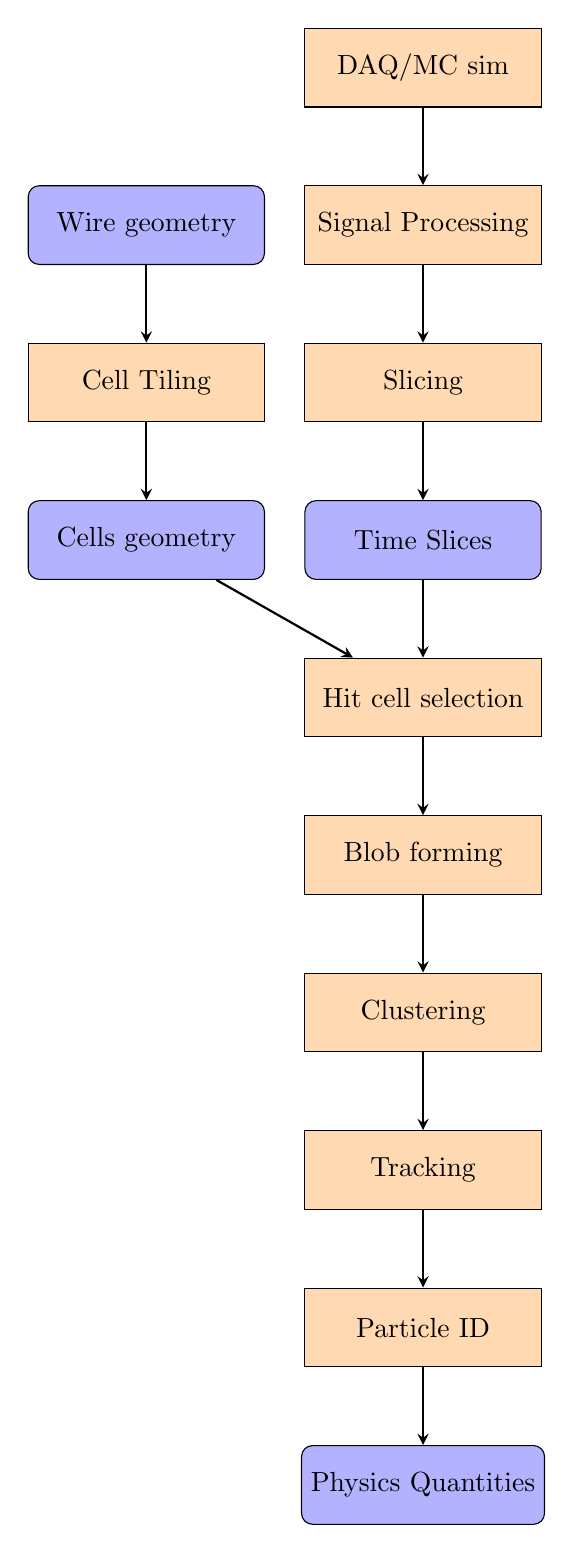
\begin{tikzpicture}[align=center, node distance=2cm]

\tikzstyle{dataobj} = [rectangle, rounded corners, minimum width=3cm, minimum height=1cm,text centered, draw=black, fill=blue!30]
\tikzstyle{process} = [rectangle, minimum width=3cm, minimum height=1cm, text centered, draw=black, fill=orange!30]
\tikzstyle{decision} = [diamond, minimum width=3cm, minimum height=1cm, text centered, draw=black, fill=green!30]
\tikzstyle{arrow} = [thick,->,>=stealth]

\node (daqmc) [process,highlight=2] {DAQ/MC sim};
\node (frames) [process,highlight=2, below of=daqmc] {Signal Processing};
\node (slicing) [process,highlight=2, below of=frames] {Slicing};
\node (slices) [dataobj, below of=slicing] {Time Slices};
\node (wires) [dataobj, left=0.5cm of frames] {Wire geometry};
\node (tiling) [process,highlight=2, left=0.5cm of slicing] {Cell Tiling};
\node (cells) [dataobj, left=0.5cm of slices] {Cells geometry};
\node (hitcells) [process,highlight=3, below of=slices] {Hit cell selection};
\node (blobbing) [process,highlight=3, below of=hitcells] {Blob forming};
\node (clustering) [process,highlight=4, below of=blobbing] {Clustering};
\node (tracking) [process,highlight=4, below of=clustering] {Tracking};
\node (pid) [process,highlight=5, below of=tracking] {Particle ID};
\node (physics) [dataobj, below of=pid] {Physics Quantities};

\draw [arrow] (wires) -- (tiling);
\draw [arrow] (tiling) -- (cells);
\draw [arrow] (cells) -- (hitcells);
\draw [arrow] (daqmc) -- (frames);
\draw [arrow] (frames) -- (slicing);
\draw [arrow] (slicing) -- (slices);
\draw [arrow] (slices) -- (hitcells);
\draw [arrow] (hitcells) -- (blobbing);
\draw [arrow] (blobbing) -- (clustering);
\draw [arrow] (clustering) -- (tracking);
\draw [arrow] (tracking) -- (pid);
\draw [arrow] (pid) -- (physics);
\end{tikzpicture}}
      \end{center}
    \end{column}
  \end{columns}

\end{frame}

\subsection{Data Preparation}

\begin{frame}
  \frametitle{Framing}
  
  \vspace{-25mm}
  \begin{center}
    \rotatebox{-90}{\includegraphics[width=6cm]{framing.pdf}}    
  \end{center}

  \vspace{-10mm}

  \scriptsize
  Wire Cell \textbf{input is raw data stream}:  $\sim$\SI{4}{\milli\second} \textbf{frames of time} (\SI{2}{\mega\hertz}, 12 bit).

  \vspace{2mm}

  \begin{columns}
    \begin{column}{0.4\textwidth}
      \scriptsize
      \textbf{MicroBooNE:}
      \begin{itemize}
      \item At FNAL, nearby computing infrastructure.
      \item \textbf{Very active at surface}: \\
        $\sim$20 cosmic-$\mu$ tracks/frame.
      \item Very ``few'' channels (8256).
      \item \textbf{full-stream} readout frames:\\
        \textbf{$\sim$120 MB/frame}.
      \end{itemize}

    \end{column}
    \begin{column}{0.6\textwidth}
      \scriptsize
      
      \textbf{DUNE:}
      \begin{itemize}
      \item \textbf{Deep underground}:\\ power/cooling/space are at a premium.
      \item \textbf{1.5M channels} could produce: \\
        5 TB/second \textbf{full-stream}!
      \item DUNE must \textbf{zero-suppress} waveforms.
      \item \textbf{$\sim$2.5 MB/frame} (25 GB if no ZS!)
      \item Isolated $^{39}$Ar decays are dominant bkg.
        \begin{itemize}\scriptsize
        \item[$\rightarrow$] requires \textbf{clever DAQ!}
        \end{itemize}
      \end{itemize}

    \end{column}
  \end{columns}
\end{frame}

\begin{frame}[fragile]
  \frametitle{Time Slicing}
  
  \begin{columns}
    \begin{column}{0.35\textwidth}
      \begin{center}
        \vspace{-.5cm}

        \includegraphics[width=\textwidth]{slice.pdf}

        \vspace{-2cm}

        \includegraphics[width=\textwidth,trim=0cm 10cm 0cm 0cm,clip]{slice-3D.pdf}

        \scriptsize One \textbf{time slice} along a plane transverse to the drift.
      \end{center}
    \end{column}
    \begin{column}{0.65\textwidth}

      \includegraphics[width=\textwidth]{wires-and-true-hits.png}

      \begin{itemize} \scriptsize
      \item Shows ``true'' (simulated) \textcolor{blue}{drifting charge}.
      \item Select \textcolor{red}{wires hit} in the slice.\\
        $\rightarrow$ hit = FADC charge-in-slice above a threshold.
      \item Slice duration is chosen to \textbf{match
          electronics shaping time}: 4 FADC ``ticks'' =
        \SI{2}{\micro\second}.
      \end{itemize}
    \end{column}
  \end{columns}

\end{frame}

\subsection{Imaging Of Activity}

\begin{frame}[fragile]
  \frametitle{Tiling}

  \vspace{-5mm}

  \begin{center}
    \scriptsize Zoom in on the wires and their associated (constructed) cells.

    \includegraphics[width=0.7\textwidth,trim=8.6cm 9cm 8.6cm 9cm,clip]{test_boundcells.pdf}

    MicroBooNE geometry shown.
  \end{center}

  \vspace{-5mm}

  \footnotesize
  Cell construction:
  \begin{itemize}
  \item Define small, 2D regions near \textit{approximate triple crossings} of one wire from each of the three planes.
  \item A ``cell'' is the association of this region with the three wires. 
  \item Cells completely tile the plane (time slice): no gaps, no overlaps.
  \item Bipartite cell types: \textit{wire-centered} and \textit{gap-centered} cells.
  \item In general (eg, DUNE), cell shapes and sizes not uniform nor regular,
    depend on wire plane pitches, angles and offsets.
  \end{itemize}

  \textbf{The heart of the Wire Cell concept:} if all three
  triple-crossing \textbf{wires} are ``hit'', the associated \textbf{cell} likely
  contains drifted charge.

\end{frame}

\begin{frame}
  \frametitle{Cell Ambiguity - Example Hit Pattern}

  \begin{columns}
    \begin{column}{0.35\textwidth}
      \begin{center}
        \scriptsize Zoom in on $5 \times 5 \times 3$ wires:

        \includegraphics[width=\textwidth,trim=3.5cm 6cm 5cm 3cm,clip]{example-hit-cells.pdf}        

        \tiny (assume just wire-centered cell def. here)
      \end{center}
    \end{column}
    \begin{column}{0.65\textwidth}

      Spatial multiplexing $\Rightarrow$ \textbf{ambiguity}:

      \vspace{5mm}

      \begin{description}\scriptsize
      \item[Good] wire \textcolor{blue}{v3} measures no charge, \\$\therefore$ all its cells must not be hit.
      \item[Bad] hits \textbf{c2}, \textbf{c7} and \textbf{c8} induce ``ghost'' at \textbf{c4}.
      \item[Ambiguous] multiple cells measured by same wire.\\
        How much charge is in \textbf{c6}???
      \end{description}

      \vspace{5mm}

      In some cases ambiguity can not be resolved at the cell level!

    \end{column}
  \end{columns}
\end{frame}

\begin{frame}[fragile]
  \frametitle{Solution Attempt 1 - cell-level}
  Expected charge measured on \textbf{wires} ($\vec{w}$) can be calculated
  knowing (unknown) charge in \textbf{cells} ($\vec{c}$):

  \[\vec{w} = \mathbf{G_{wc}}\vec{c}\]

  $\mathbf{G_{wc}}$ is the \textbf{wire-cell adjacency matrix}, purely
  geometrical and perfectly known, function of detector design.
  
  \begin{columns}
    \begin{column}{0.45\textwidth}
      \vspace{-5mm}

      \flushright \includegraphics[width=0.8\textwidth,trim=1cm 11cm 2cm 2cm,clip]{example-hit-cells.pdf}

    \end{column}
    \begin{column}{0.10\textwidth}
      $\Leftrightarrow$
    \end{column}
    \begin{column}{0.45\textwidth}

  \resizebox{0.7\textwidth}{!}{
    $\left(
      \begin{array}[h]{c}
        0.0\\
        1.0\\
        2.0\\
        2.0\\
        0.0\\

        1.0\\
        1.0\\
        0.0\\
        2.0\\
        1.0\\

        1.0\\
        2.0\\
        2.0\\
      \end{array}
    \right)
    = \left(
      \begin{array}[h]{ccccccccc}
        1&0&0&0&0&0&0&0&0\\
        0&1&0&1&0&0&0&0&0\\
        0&0&1&0&1&0&1&0&0\\
        0&0&0&0&0&1&0&1&0\\
        0&0&0&0&0&0&0&0&1\\

        0&0&0&0&0&0&1&0&0\\
        0&0&0&1&0&0&0&1&0\\
        1&0&0&0&1&0&1&0&0\\
        0&1&0&0&0&1&0&0&0\\
        0&0&1&0&0&0&0&0&0\\
        
        1&0&0&1&0&0&1&0&0\\
        0&1&0&0&1&0&0&1&0\\
        0&0&1&0&0&1&0&0&1\\
      \end{array}
    \right)
    \left(
      \begin{array}[h]{c}
        0.0\\
        1.0\\
        1.0\\
        0.0\\
        0.0\\
        1.0\\
        1.0\\
        1.0\\
        0.0\\
      \end{array}
    \right)$}
      
    \end{column}
  \end{columns}


  Wish to solve inverse: $\vec{c} = \mathbf{G}^{-1}_{\mathbf{wc}}\vec{w}$.
  However, $N_{cells} \approx N_{wires}^2$ \\
  $\Rightarrow$ as $N_{cells}$ grows, more unknowns ($\vec{c}$) than knowns ($\vec{w}$)!
\end{frame}

\begin{frame}
  \frametitle{Solution Attempt 2 - blob-level}
  \vspace{-10mm}
  \begin{columns}
    \begin{column}{0.6\textwidth}
      Goal: \textbf{reduce matrix size} and \textbf{remove ambiguity} by making ``blobs'' of cells.
    \end{column}
    \begin{column}{0.4\textwidth}
      \includegraphics[width=0.8\textwidth]{wires-and-true-hits.png}          
    \end{column}
  \end{columns}
      
  \begin{enumerate}
  \item Select set of all cells with all three wires ``hit''.
  \item Partition set into spatially contiguous subsets: ``\textbf{blobs}''.
  \end{enumerate}
  Equation to solve is now:
  \[\vec{w_b} = \mathbf{G_{wb}} \vec{b}\]

  \begin{description}
  \item[$\vec{c} \to \vec{b}$] vector of charge in each blob.
  \item[$\mathbf{G_{wc}} \to \mathbf{G_{wb}}$] the wire-blob adjacency matrix for the slice.
  \item[$\vec{w} \to \vec{w_b}$] vector of charge on all wires associated with a blob.
  \end{description}

\end{frame}

% maybe remove this slide...
\begin{frame}
  \frametitle{Another wrinkle: charge uncertainty}

  Measure of the drifting charge by a wire has uncertainty:
  \begin{itemize}
  \item Environmental, electronic and thermal noise.
    \begin{itemize}\footnotesize
    \item[$\rightarrow$] Can be correlated across wires.
    \end{itemize}
  \item Statistical uncertainty due to digitization.
  \item Systematic uncertainties from detector response deconvolution.
  \end{itemize}
  Compare measured wire charge ($\vec{w}_{meas}$) with expected
  ($\vec{w}_{exp}$) and form a $\chi^2$ with $\mathrm{V}$ a
  covariance uncertainty matrix.
  
  \[\chi^2 = (\vec{w}_{meas}-\vec{w}_{exp})^\intercal\mathrm{V}^{-1} (\vec{w}_{meas}-\vec{w}_{exp})\]

  ``It can be shown'' that minimizing this $\chi^2$ is equivalent to
  inverting $\mathbf{G_{wc}}$ (or $\mathbf{G_{wb}}$) matrix equation.


  \begin{center}
    \textbf{$\rightarrow$ This is a very CPU intensive, but critical step!}
  \end{center}

\end{frame}

\begin{frame}[fragile]
  \frametitle{The Payoff: imaged \SI{3}{\giga\electronvolt} $\nu_e$ interaction}
  
  \begin{columns}
    \begin{column}{0.5\textwidth}
      \begin{center}
        \includegraphics[width=\textwidth,trim=3cm 10cm 3cm 10cm,clip]{payoff-true.png}

        True energy depositions.
      \end{center}
    \end{column}
    \begin{column}{0.5\textwidth}
      \begin{center}
        \includegraphics[width=\textwidth,trim=3cm 10cm 3cm 10cm,clip]{payoff-reco.png}

        Wire Cell Imaging.
      \end{center}
    \end{column}
  \end{columns}

  \vfill

  \footnotesize
  \begin{itemize}
  \item Excellent imaging of major track features as well as isolated
    activity.
    \begin{itemize}\scriptsize
    \item[$\rightarrow$] a static 2D view doesn't do it justice!  \href{http://www.phy.bnl.gov/wire-cell/bee/set/6/event/0/}{See it for yourself.}
    \end{itemize}
  \item Remaining ambiguity seen as wide blue patches.
    \begin{itemize}\scriptsize
    \item[$\rightarrow$] inherent in LArTPC technology, Wire Cell just makes it evident.
    \item[$\rightarrow$] battling this will likely require CPU-intensive algorithms and/or relying on iterative reconstruction.
    \end{itemize}
  \end{itemize}
\end{frame}


\subsection{Pattern Recognition}

\begin{frame}
  \frametitle{Clustering, Tracking and Categorization}
  Post-imaging, current approach:
  \begin{enumerate}
  \item \textbf{cluster} together blobs contiguous in space and time
    (slice).
  \item \textbf{track} a line through a cluster.
  \item \textbf{categorize} success/failure of line to account for the
    cluster's charge distribution.
  \end{enumerate}
  Some categories:
  \begin{description}
  \item[track] cluster is well fit by the track
  \item[short] cluster appears to be a ``short track'' (eg, $\delta$-ray)
  \item[shower] cluster appears to be a EM/hadronic shower
  \item[undefined] no well-suited categorization.
  \end{description}

  \begin{itemize}
  \item Active area of Wire Cell development.
  \item May benefit from collaboration with machine learning experts. 
  \end{itemize}

\end{frame}

\subsection{Physics}
\begin{frame}
  \frametitle{Physics-level Reconstruction}

  This development is just beginning.
  
  It will:
  \begin{itemize}
  \item associate clusters with a particle trajectory
  \item determine particle type
  \item determine momentum, range, dE/dx and other kinematics.
  \end{itemize}

\end{frame}


\section{Software Design}

\begin{frame}
  \tableofcontents[currentsection,hideothersubsections]
\end{frame}


\begin{frame}
  \frametitle{Wire Cell Software Ecosystem}

  Wire Cell breaks up into three main parts:

  \begin{description}
  \item[visualization] the ``Bee'' web application (Chao Zhang)
  \item[prototype] reconstruction algorithms, initial proof of
    principle (Xin Qian)
  \item[toolkit] ``production'' toolkit for LArTPC reconstruction (bv)
  \end{description}

\end{frame}

\subsection{Bee Display}

\begin{frame}
  \frametitle{Bee: an interactive 3D visualization system}

  \textbf{Bee} features:
  \begin{itemize}
  \item Displays results of different reconstruction algorithms.
  \item Shows ``true'' particle trajectories from simulation.
  \item Very good for developers to debug and compare different
    methods and for users to gain Physics/LArTPC intuition.
  \item Implemented in \textbf{JavaScript/WebGL} + \textbf{Django}.
  \item Works on popular desktop and mobile browsers.
  \item Requires hardware WebGL support.
  \item JSON data file format, easy to implement schema.
  \item Supports drag-and-drop
    \href{http://bnlif.github.io/wire-cell-docs/viz/uploads/}{user
      file uploads}.
  \item New features almost daily (\textbf{Chao Zhang}!)
  \end{itemize}
\end{frame}

\begin{frame}[fragile]
  \frametitle{Bee: Select and upload event sets}
  \begin{center}
    \includegraphics[height=0.8\textheight]{bee-event-sets-page.png}

    \vspace{-3cm}
    \flushright \footnotesize Simple JSON format\\
    \includegraphics[width=3cm]{json-data.png}
  \end{center}
\end{frame}

\begin{frame}
  \frametitle{Interactive 3D visualization}
  \begin{center}
    \includegraphics[height=0.7\textheight]{bee-full-gui.png}    
  \end{center}
  \begin{center}
    Try it yourself! \url{http://www.phy.bnl.gov/wire-cell/bee/}
  \end{center}
\end{frame}


\subsection{Prototype}

\begin{frame}
  \frametitle{Wire Cell Working Prototype}
  \footnotesize

  \begin{itemize}
  \item \textbf{Very successful proof of principle!}
  \item Currently \textbf{leads the state of the art} in LArTPC
    reconstruction techniques.
  \item Amazingly fast development (\textbf{Xin Qian}!)
    \begin{itemize}\scriptsize
    \item[$\rightarrow$] Work started only $\sim$5 months ago!
    \end{itemize}
  \end{itemize}

  \begin{center}
    \includegraphics[height=0.5\textheight,trim=0cm 0cm 0cm 2cm,clip]{xin-shower.png}

    \scriptsize
    Colors indicate identified tracks and showers.
  \end{center}

\end{frame}

\begin{frame}
  \frametitle{Compromises to Remedy}

  Some compromises were accepted for the rapid prototype and now need
  ``back-filling''.  Need to remedy:

  \begin{itemize}
  \item No support for long-term, multi-developer contributions.
  \item Many monolithic, single-threaded applications.
  \item Hard-coded ``magic'' numbers $\to$ configuration.
  \item Rigid code structure and hard-coded workflows.
  \item External software integrated only through file exchange.
  \item Need comprehensive CPU/memory optimization campaign.
  \item Some high-level tests, need coverage/granularity.
  \item Intimate dependency on the large
    ROOT\footnote{\url{https://root.cern.ch/}} toolkit.
  \end{itemize}

  Decision: rewrite rather than refactor $\longrightarrow$
  
\end{frame}

\subsection{Toolkit}

\begin{frame}
  \frametitle{Wire Cell Toolkit}
  \begin{columns}
    \begin{column}{0.65\paperwidth}
    \end{column}
    \begin{column}{0.35\paperwidth}
      \vspace{-20mm}
      \includegraphics[width=\textwidth]{deps.pdf}      
    \end{column}
  \end{columns}

  \vspace{-15mm}

  High level overview:
  \begin{itemize}
  \item Includes \textbf{packaging and build} system.
  \item Comprehensive \textbf{API} via abstract base classes.
  \item Mindful of \textbf{dependencies}, external and internal.
  \item Built-in wire and cell \textbf{geometry descriptions} or load from file.
  \item Includes simple \textbf{LArTPC detector simulation}.
  \item Rewrite implementations of core \textbf{prototype algorithms}.
  \item Abstracted \textbf{execution model}, step towards parallelism.
  \item Support for native and foreign \textbf{file I/O}.
  \item Follow ``\textbf{toolkit}'' software paradigm.
  \end{itemize}

  \vfill

  Good progress along all fronts but still much work to do.

\end{frame}

\begin{frame}[fragile]
  \frametitle{Source Repositories and Build}

  \begin{itemize}
  \item Code in GitHub \href{https://github.com/WireCell/}{WireCell} organization.
  \item Code aggregation with \textbf{git submodule}.
  \item A simple, customized \href{https://waf.io/}{waf}-based build.\footnote{\texttt{wcb} = \texttt{waf} + extra Waf tools for Boost, ROOT, Eigen and Wire Cell packaging}
  

  \end{itemize}

  \begin{lstlisting}{langauge=shell}
$ git clone git@github.com:WireCell/wire-cell.git
$ cd wire-cell/
$ git submodule init
$ git submodule update
$ ./wcb --prefix=/path/to/install configure build install
  \end{lstlisting}
%$

  Builds, tests and installs:
  \begin{itemize}
  \item toolkit shared libraries + header files,
  \item no main applications yet but many, unit+integration tests
  \end{itemize}
  Also: \href{http://www.phy.bnl.gov/wire-cell/doxy/html/}{Doxygen reference} and \href{http://wirecell.github.io/wire-cell-docs/}{MkDocs user documentation}.


\end{frame}

\begin{frame}[fragile]
  \frametitle{Wire Cell Interfaces}

  The \href{https://github.com/WireCell/wire-cell-iface}{\texttt{wire-cell-iface}} package:

  \begin{itemize}
  \item API composed of abstract base classes covering:
    \begin{itemize}
    \item \textbf{Data model} (wires, cells, frames, slices, tracks, ...)
    \item \textbf{Active components} (blob maker, matrix solver, clustering, ...)
    \end{itemize}
  \item Pervasive use of C++ \verb|shared_ptr<>| for (mostly) \textbf{worry-free memory management}.
  \item Dynamic instance lookup via \texttt{NamedFactory} pattern
    allows for a \textbf{plugin architecture}.
  \item Initial support for \textbf{user configuration} system based on Boost
    property trees.
  \item Initial support exists for an \textbf{abstract execution model}.
    \begin{itemize}\scriptsize
    \item[$\rightarrow$] more on this coming up.
    \end{itemize}
  \end{itemize}
\end{frame}

\begin{frame}

  \frametitle{Wire Cell Simulation}

  \begin{columns}
    \begin{column}{0.75\textwidth}
      \begin{itemize}\footnotesize
      \item Provided by the \href{https://github.com/WireCell/wire-cell-gen}{\texttt{wire-cell-gen}} package.
      \item Simple implementation of the 4 ``D''s of LArTPC:\\
        \textbf{deposit, drift, diffuse, digitize}.
      \item Granular, use as little or as much as needed.
        \begin{itemize}\scriptsize
        \item[$\rightarrow$] Parts can be replaced by external
          simulation, \\or bypassed entirely with real DAQ data.
        \item[$\rightarrow$] External integration via file I/O or API calls.
        \end{itemize}
      \item Provides reference implementation to guide integrator/developers of external frameworks.
      \item Useful for quickly generating data to feed unit tests.
      \end{itemize}
    \end{column}
    \begin{column}{0.25\textwidth}
      \vspace{-10mm}
      \includegraphics[width=\textwidth]{sim-flow.pdf}
    \end{column}
  \end{columns}
\end{frame}

\begin{frame}[fragile]
  \frametitle{Wire Cell Execution Model}

  \begin{columns}
    \begin{column}{0.7\textwidth}
      \footnotesize 
      The toolkit supports \textbf{data flow programming} paradigm
      \begin{itemize}
        \item Design directly influenced by
          \href{http://www0.bnl.gov/events/details.php?q=8932}{CSC Seminar on VisTrails, March 2013}!
        \item Data flows through a graph made from:
          \begin{description}
          \item[vertices:] computational units / algorithms
          \item[edges:] data queues of a given type
          \end{description}
        \item Each queue carries well defined data types.
        \item Streamed processing minimizes RAM usage.
        \item Graph-level ``programming'' to define workflows.
        \item Thread-safe queues $\Rightarrow$ parallel processing.
        \item Graph execution machinery swapable: uniproc, multiproc, or
          distributed (MPI) parallel.
        \item Encourages isolated, targeted development and testing of each
          compute vertex.
        \item Feedback loops to implement iterative workflows.
        \item Instrument graph to collect performance data.
        \end{itemize}
      \end{column}
      \begin{column}{0.3\textwidth}

        \vspace{-10mm}

        \includegraphics[width=\textwidth]{dataflow.pdf}

        \tiny One possible high-level flow.
      \end{column}
    \end{columns}
\end{frame}

\begin{frame}
  \frametitle{Abstract execution model}

  \scriptsize Want ability to change execution model while leaving ``real'' algorithm code untouched!

\footnotesize
  
  \begin{columns}
    \begin{column}{0.6\textwidth}
      Each graph vertex made from \textbf{three layers}.\\
      From outside to in:
      \begin{enumerate}
      \item Execution model layer implementing data flow control
        \begin{itemize}\scriptsize
        \item sync'ed load-and-flush, async, multi-processing, message-passing, ...
        \end{itemize}
      \item Adapter wraps actual algorithm and matches to a uniform execution model interface.
      \item Algorithm implementation and interface left unrestricted
        except ``no shared globals'' (thread safety).
      \end{enumerate}
    \end{column}
    \begin{column}{0.4\textwidth}
      \includegraphics[width=1.1\textwidth]{concentric.pdf}      
    \end{column}
  \end{columns}

\end{frame}

\section{Future Plans}

\begin{frame}
  \tableofcontents[currentsection,hideothersubsections]
\end{frame}

\begin{frame}\frametitle{Future Plans}
  \begin{center}
    ...in which I frequently beg for help : )
  \end{center}
\end{frame}

\subsection{Algorithm Development}

\begin{frame}
  \frametitle{Pattern Recognition}
  Pattern recognition stage is turning out to be ``hard''.
  \footnotesize
  \begin{itemize}
  \item Many challenges are \textbf{inherent to the LArTPC technology}.  
    \begin{itemize}\scriptsize
    \item[$\rightarrow$] Wire Cell has just allowed us to reach them.
    \end{itemize}
  \item Current implementation is largely \textbf{heuristic based}
    \begin{itemize}\scriptsize
    \item many ``cross-algorithm assumptions''
    \item \textbf{large solution space} with \textbf{many corner cases}.
    \item human Physicists find good but \textbf{per-event/ad-hoc solutions}.
    \item[$\rightarrow$] how to teach them to the computer?
    \end{itemize}
  \item[$\rightarrow$] Our attempt: Bee 2.0 (next slide) 
  \end{itemize}
  
  \vfill

  We have a few ideas but we feel we may be entering to the area of ``real'' computer science
  problems like \textbf{machine learning} and maybe \textbf{machine vision}.

  \vspace{2mm}

  And we are not experts. 

  \vspace{2mm}

  \textbf{Help Wanted!}

\end{frame}

\subsection{Bee 2.0}


\begin{frame}
  \frametitle{Bee 2.0: Human-directed Automated Reconstruction}
  Interim Solution: inject human judgment to guide pattern recognition.
  \begin{enumerate}
  \item Bee will let humans \textbf{interactively inject commands}, eg:
    \begin{enumerate}
    \item ``Join cluster X to cluster Y''
    \item ``Remove blob AAA from cluster Z''
    \item ``Now, rerun automatic reconstruction''
    \end{enumerate}
  \item Convert human commands into operational objects.
  \item Send to back-end, execute inside a Wire Cell service.
  \item Send results back to user.
  \item Record everything in a database to mine for potential Wire
    Cell improvements.
  \end{enumerate}
  Think: ``\textbf{Physics-PhotoShop}'' + ``\textbf{Google Analytics}''.

\end{frame}

\begin{frame}
  \frametitle{Bee 2.0: Architecture}
  Architectural plans include:
  \begin{itemize}
  \item Move Bee from \href{http://threejs.org/}{\texttt{three.js}} to a new JS/WebGL framework to support interactive controls (eg ``picking'').
  \item Develop a web-friendly \textbf{batch workflow system} (probably based on Celery) to run Wire Cell promptly.
  \item Develop a \textbf{database} system to capture ``analytics'' and coordinate the system (likely to use MongoDB).
  \item Further develop the Django \textbf{middleware} to tie it together.
  \item Provision the \textbf{hardware} to support/run all of this (\textbf{at BNL}).
  \end{itemize}

  \vfill

  Ideas are still early but conceptually it is a \textbf{rather big} system.

  \vfill

  \textbf{Help wanted!}

\end{frame}

\subsection{Parallel Wire Cell}

\begin{frame}
  \frametitle{Wire Cell Production Processing}

  A 1-2 punch for today's computing:
  \begin{itemize}\footnotesize
  \item[$\rightarrow$] Need high thoughput to keep up with detector data rates.
  \item[$\rightarrow$] Need high performance due to CPU-heavy algorithms.
  \end{itemize}

  \footnotesize

  \begin{columns}
    \begin{column}{0.70\textwidth}
      Data volumes:
      \begin{description}
      \item[MicroBooNE] $\sim$630 TB/year (compressed)
      \item[protoDUNE] $\mathcal{O}$(1PB) total, (ZS, uncomp.)
      \item[DUNE 40kt] $\mathcal{O}$(PB)/year (ZS, uncomp.)
      \end{description}
      \begin{itemize}
      \item Okay, it's not quite ATLAS-levels 
        \begin{itemize}\scriptsize
        \item Run 1 produced $\sim$3PB/year raw.
        \end{itemize}
      \item But: \textbf{Wire Cell needs raw wire data} as input
        \begin{itemize}\scriptsize
        \item No Level-X triggers to save you.
        \item MicroBooNE: offline sees full-stream, no-ZS.
        \item Surface protoDUNE: $\sim$60 cosmic-$\mu$s per readout.
        \item Underground DUNE: all detector activity is sacred.
        \end{itemize}
      \item Current speed: \textbf{30 minutes -- 1day / event!}
        \begin{itemize}\scriptsize
        \item Major caveat: some optimization expected, will
          paralleize, etc, etc, but: \textbf{*GULP*!}
        \end{itemize}
      \end{itemize}
    \end{column}
    \begin{column}{0.30\textwidth}
      \begin{center}
        \includegraphics[width=\textwidth,trim=5cm 9cm 3cm 6cm,clip]{frank-abuse.pdf}

        \scriptsize (with apologies to \href{https://www.bnl.gov/events/details.php?q=11000}{Frank Wuerthwein})
      \end{center}
    \end{column}
  \end{columns}

\end{frame}

\begin{frame}
  \frametitle{Taking Wire Cell Parallel}

  Parallel processing plans mostly involve implementing different
  execution models:

  \begin{enumerate}\footnotesize
  \item \href{https://github.com/erenon/pipeline}{Boost.Pipeline} nice
    and simple threaded data flow package.  Easy to start with but not
    yet officially part of BOOST (longevity concerns?).
  \item \href{https://www.threadingbuildingblocks.org/}{Intel TBB} a
    common and well supported library with a fantastic looking ``flow
    graph designer'' tool.  Some effort needed to learn/adopt.
  \item MPI/ZeroMQ or other ways to run Wire Cell as multiple-node
    distributed process (maybe on \textbf{HPC}).  Big learning curve
    for us.
  \item Also, investigate potential for \textbf{GPU/Phi} hardware
    acceleration of particular bottlenecks. Even bigger learning curve!
  \end{enumerate}

  \vfill

  This level of parallelism is \textbf{new ground for us}\footnote{This is a subject of a pending BNL/Computing LDRD proposal.}.

  \vfill

  \textbf{Help wanted!}
\end{frame}


\section{}

\begin{frame}
  \frametitle{Summary}
  \footnotesize
  \begin{itemize}
  \item The \textbf{Wire Cell working prototype LArTPC reconstruction} method and software has been developed.
    \begin{itemize}  \footnotesize
    \item already producing some of the \textbf{world's best results},
    \item technical and performance improvements still needed.
    \end{itemize}
  \item The \textbf{Bee interactive 3D event visualization}
    application developed, critical for understanding LArTPC and
    developing Wire Cell.  Plans to evolve to ``human-directed
    automated reconstruction''.
  \item The \textbf{Wire Cell Toolkit} for LArTPC reconstruction
    partly complete and will be the basis for long term development
    including investigations into parallel processing.
  \item To be successful we are going into \textbf{new waters} (for
    us) of parallel processing, hardware acceleration, computing
    science and mathematics.
  \end{itemize}

  \begin{center}
    $\rightarrow$ \textbf{Expert input, help and collaboration are most welcome!}
  \end{center}
\end{frame}

\begin{frame}
  \frametitle{Wire Cell on the web}

  \begin{itemize}
  \item home page: \\ \url{http://www.phy.bnl.gov/wire-cell/}
  \item Bee entry: \\ \url{http://www.phy.bnl.gov/wire-cell/bee/}
  \item prototype user manual: \\ \url{http://bnlif.github.io/wire-cell-docs/}
  \item toolkit user manual: \\ \url{http://wirecell.github.io/wire-cell-docs/}
  \item toolkit reference: \\ \url{http://www.phy.bnl.gov/wire-cell/doxy/html/}
  \item prototype repositories: \\ \url{https://github.com/BNLIF}
  \item toolkit repositories: \\ \url{https://github.com/WireCell}
  \end{itemize}
\end{frame}

\end{document}


%%% Local Variables:
%%% mode: latex
%%% TeX-master: t
%%% End:
